% Presenter info: 
% http://www.linuxclustersinstitute.org/Linux-HPC-Revolution/presenterinfo.html
%
% Main Text Layout
% Set the main text in 10 point Times Roman or Times New Roman (normal), 
% (no boldface), using single line spacing. All text should be in a single 
% column and justified. 
%
% Opening Style (First Page)
% This includes the title of the paper, the author names, organization and 
% country, the abstract, and the first part of the paper.
% * Start the title 35mm down from the top margin in Times Roman font, 16 
%   point bold, range left. Capitalize only the first letter of the first 
%   word and proper nouns.
% * On a new line, type the authors' names, organizations, and country only 
%   (not the full postal address, although you may add the name of your 
%   department), in Times Roman, 11 point italic, range left.
% * Start the abstract with the heading two lines below the last line of the 
%   address. Set the abstract in Times Roman, 12 point bold.
% * Leave one line, then type the abstract in Times Roman 10 point, justified 
%   with single line spacing.
%
% Other Pages
% For the second and subsequent pages, use the full 190 x 115mm area and type 
% in one column beginning at the upper right of each page, inserting tables 
% and figures as required.
% 
% We're recommending the Lecture Notes in Computer Science styles from
% Springer Verlag --- google on Springer Verlag LaTeX.  These work nicely,
% *except* that it does not work with the hyperref package. Sigh.
%
% http://www.springer.de/comp/lncs/authors.html
%
% NOTE: This is an excerpt from the document in slurm/doc/pubdesign

\documentclass[10pt,onecolumn,times]{../common/llncs}

\usepackage{verbatim,moreverb}
\usepackage{float}

% Needed for LLNL cover page / TID bibliography style
\usepackage{calc}
\usepackage{epsfig}
\usepackage{graphics}
\usepackage{hhline}
\input{pstricks}
\input{pst-node}
\usepackage{chngpage}
% ***************** llnlCoverPage.tex ********************************************************************************
% This file defines the following commands for generating the
% front and back cover pages:
%
%     \makeLLNLCover{UCRL}{Title}{Authors}{Journal}{Date}{hShift}{vShift}
%  and
%     \makeLLNLBackCover
%
% where
%
%  UCRL: The UCRL (6 digit) number (which you probably won't know before the document
%        is released so just make up a number)
%  Title: title of the article
%  Authors: Authors separated by \\
%  Journal: The journal name
%  Date : the date
%  hShift,vShift : horizontal and vertical shifts to apply to the title page to position it correctly (since
%                  the automatic positioning may not work)
%
% Here is an example:
%  \makeLLNLCover{123456}{An adaptive numerical method for high-speed reactive flows}{William D. Henshaw\\%
%   Donald W. Schwendeman}{Journal of Computational Physics}{January 1, 2003}{0in}{0in}
%
% *****************************************************************************************************************
%
\newcommand{\setPageForLLNLCover}[2]{%
\newlength{\textwidthOld}%
\setlength{\textwidthOld}{\textwidth}%
\newlength{\textheightOld}%
\setlength{\textheightOld}{\textheight}%
\newlength{\topmarginOld}%
\setlength{\topmarginOld}{\topmargin}%
\newlength{\textwidthNew}%
\setlength{\textwidthNew}{6.5in}%
\newlength{\textheightNew}%
\setlength{\textheightNew}{9.5in}%
\newlength{\oddsidemarginNew}%
\newlength{\topmarginNew}%
\setlength{\oddsidemarginNew}{(\paperwidth-\textwidthNew)/2 - 1in + #1}%
\setlength{\topmarginNew}{(\paperheight-\textheightNew -\headheight-\headsep-\footskip)/2 - 1in +1.cm + #2}%
\newlength{\oddsidemarginOld}%
\setlength{\oddsidemarginOld}{\oddsidemargin}%
\changepage{\textheightNew-\textheightOld}{\textwidthNew-\textwidthOld}{\oddsidemarginNew-\oddsidemarginOld}{\oddsidemarginNew-\oddsidemarginOld}{}{\topmarginNew-\topmarginOld}{}{}{}%
}%
\newcommand{\setPageForLLNLBackCover}{%
\changepage{\textheightNew-\textheightOld}{\textwidthNew-\textwidthOld}{\oddsidemarginNew-\oddsidemarginOld}{\oddsidemarginNew-\oddsidemarginOld}{}{\topmarginNew-\topmarginOld}{}{}{}%
}%
\newcommand{\resetPageFromLLNLCover}{%
\changepage{-\textheightNew+\textheightOld}{-\textwidthNew+\textwidthOld}{-\oddsidemarginNew+\oddsidemarginOld}{-\oddsidemarginNew+\oddsidemarginOld}{}{-\topmarginNew+\topmarginOld}{}{}{}%
}%
% *************************************************************************************


% *************************************************************************************
\newcommand{\makeLLNLCover}[7]{%
\setPageForLLNLCover{#6}{#7}%
\thispagestyle{empty}% no number of this page
\newcommand{\logoWidth}{1.65in}%
\psset{xunit=1.cm,yunit=1.cm,runit=1.cm}%
\begin{pspicture}(0,0)(17,24.)
% turn on the grid for placement
% \psgrid[subgriddiv=2]
\rput(2.3,12.5){
\epsfig{file=../common/Logo_for_papers.ps,width=\logoWidth}}
\rput(11.2,23.){\parbox{12.0cm}{\large\bf%
\begin{flushright}
% jg - just pass in full UCRL string
%Preprint \\
%UCRL-JC-#1
#1
\end{flushright}
}}
\rput(10.5,18){\parbox{12.0cm}{%\sffamily\bfseries\Huge\noindent%
\fontsize{24.88}{30pt}\usefont{OT1}{cmss}{bx}{n}
\begin{flushleft}
#2
\end{flushleft}
}}
\rput(10.5,13.){\parbox{12.0cm}{%\sffamily\LARGE\noindent%
\fontsize{17.28}{18pt}\usefont{OT1}{cmss}{m}{sl}
\begin{flushleft}
#3
\end{flushleft}
}}
\rput(10.5,9.5){\parbox{12.0cm}{% \sffamily\large\noindent%
\fontsize{14}{16pt}\usefont{OT1}{cmss}{m}{n}
This article was submitted to #4
}}
\rput(10.5,7.5){\parbox{12.0cm}{% \sffamily\bfseries\LARGE\noindent%
\fontsize{20.74}{22pt}\usefont{OT1}{cmss}{bx}{n}
\begin{flushleft}
#5
\end{flushleft}
}}
% \rput[l](4,6.375){\psframebox{\parbox{2.5cm}{\bf%
% \begin{flushleft}
% Lawrence\\
% Livermore\\
% National\\
% Laboratory
% \end{flushleft}
% }}}
\rput(10.5,-1.){\parbox{12.0cm}{%
Approved for public release; further dissemination unlimited}}
\end{pspicture}
% }
%
\clearpage
% -------------- back of front cover -------------------------
\changetext{.625in}{}{}{}{}
\thispagestyle{empty}% no number of this page
\vglue5\baselineskip
\begin{center}
{\bf DISCLAIMER}
\end{center}
\noindent
% jg - updated disclaimer for report format
This document was prepared as an account of work sponsored by an
agency of the United States Government.  Neither the United States
Government nor the University of California nor any of their
employees, makes any warranty, express or implied, or assumes any
legal liability or responsibility for the accuracy, completeness, or
usefulness of any information, apparatus, product, or process
disclosed, or represents that its use would not infringe privately
owned rights. Reference herein to any specific commercial product,
process, or service by trade name, trademark, manufacturer, or
otherwise, does not necessarily constitute or imply its endorsement,
recommendation, or favoring by the United States Government or the
University of California.  The views and opinions of authors expressed
herein do not necessarily state or reflect those of the United States
Government or the University of California, and shall not be used for
advertising or product endorsement purposes.
\vskip2\baselineskip
\noindent
This work was performed under the auspices of the U. S. Department of
Energy by the University of California, Lawrence Livermore National
Laboratory under Contract No. W-7405-Eng-48.
\vskip1\baselineskip
\vfill
\clearpage
\changetext{-.625in}{}{}{}{}
\resetPageFromLLNLCover
\setcounter{page}{1}
% -----------------------------------------------------------------------------------
}
% *************************************************************************************


% *************************************************************************************
\newcommand{\makeLLNLBackCover}{%
\clearpage
\setPageForLLNLBackCover
% jg - suppress printing of essentially blank page here
%\changetext{.625in}{}{}{}{}
%\thispagestyle{empty}% no number of this page
\ \
%\vfill
%\begin{center}
%Approved for public release; further dissemination unlimited
%\end{center}
%\clearpage
%\clearpage
%\changetext{-.625in}{}{}{}{}
% ---------------------------------------------------------------------------
\thispagestyle{empty}% no number of this page
\renewcommand{\logoWidth}{10.in}
% \vglue\vShift
% \hglue\hShift
\begin{pspicture}(0,0)(17,24.)
% turn on the grid for placement
% \psgrid[subgriddiv=2]
\rput{90}(2.3,12.5){
\epsfig{file=../common/Rule_and_address.ps,width=\logoWidth}}
% \rput*[l]{90}(5.5,0){\psframebox{\parbox{8.0cm}{\large%
% \begin{flushleft}
% University of California\\
% Lawrence Livermore National Laboratory\\
% Technical Information Department\\
% Livermore, CA 94551
% \end{flushleft}
% }}}
\end{pspicture}
% \setlength{\textwidth}{4.in}      % page width
% \setlength{\textheight}{8.in}    % page height
\clearpage
\resetPageFromLLNLCover
% -----------------------------------------------------------------------------------
}
% *************************************************************************************






% Uncomment for DRAFT "watermark"
\usepackage{draftcopy}

% Times font as default roman
\renewcommand{\sfdefault}{phv}
\renewcommand{\rmdefault}{ptm}
%\renewcommand{\ttdefault}{pcr}
%\usepackage{times}
\renewcommand{\labelitemi}{$\bullet$}

\setlength{\textwidth}{115mm}
\setlength{\textheight}{190mm}
\setlength{\oddsidemargin}{(\paperwidth-\textwidth)/2 - 1in}
\setlength{\topmargin}{(\paperheight-\textheight -\headheight-\headsep-\footskip
)/2 - 1in + .5in }

% couple of macros for the title page and document
\def\ctit{SLURM Resource Management for Blue Gene/L}
\def\ucrl{UCRL-JC-TBD}
\def\auth{Morris Jette \\ Danny Auble \\ Dan Phung}
\def\pubdate{October 18, 2004}
\def\journal{Conference TBD}

\begin{document}

% make the cover page
%\makeLLNLCover{\ucrl}{\ctit}{\auth}{\journal}{\pubdate}{0in}{0in}

% Title - 16pt bold
\vspace*{35mm}
\noindent\Large
\textbf{\ctit}
\vskip1\baselineskip
% Authors - 11pt
\noindent\large
{Morris Jette, Dan Phung and Danny Auble \\
{\em Lawrence Livermore National Laboratory, USA}
\vskip2\baselineskip
% Abstract heading - 12pt bold
\noindent\large
\textbf{Abstract}
\vskip1\baselineskip
% Abstract itself - 10pt
\noindent\normalsize
The Blue Gene/L (BGL) system is a highly scalable computer developed 
by IBM and deployed Lawrence Livermore National Laboratory (LLNL). 
The current system has over 131,000 processors interconnected by a 
three-dimensional toroidal network with complex rules for managing 
the network and allocating resources to jobs.
SLURM (Simple Linux Utility for Resource Management ) was selected to 
fulfull this role. 
SLURM is an open source, fault-tolerant, and highly scalable cluster 
management and job scheduling system in widespread use on Linux clusters.
This paper presents overviews of BGL resource management issues and
SLURM architecture.
It also presents a description of how SLURM provides resource 
management for BGL and preliminary performance results.

% define some additional macros for the body
\newcommand{\munged}{{\tt munged}}
\newcommand{\srun}{{\tt srun}}
\newcommand{\scancel}{{\tt scancel}}
\newcommand{\squeue}{{\tt squeue}}
\newcommand{\scontrol}{{\tt scontrol}}
\newcommand{\sinfo}{{\tt sinfo}}
\newcommand{\slurmctld}{{\tt slurmctld}}
\newcommand{\slurmd}{{\tt slurmd}}
\newcommand{\smap}{{\tt smap}}

\section{Overview}

The BlueGene/L (BGL) system offers a unique cell-based design in which 
the capacity can be expanded without introducing bottlenecks 
\cite{BlueGeneWeb,BlueGeneL2002}.
The Blue Gene/L system delivered to LLNL consists of 
131,072 processors and 33TB of memory \cite{BlueGene2002}.  
The peak computational rate will exceed 360 TeraFLOPs.

Simple Linux Utility for Resource Management (SLURM)\footnote{A tip of 
the hat to Matt Groening and creators of {\em Futurama},
where Slurm is the most popular carbonated beverage in the universe.} 
is a resource management system suitable for use on both small and 
very large clusters. 
SLURM was developed by Lawrence Livermore National Laboratory
(LLNL), Linux NetworX and HP. 
It has been deployed on hundreds of Linux clusters world-wide and has 
proven both highly reliable and highly scalalble.

\section{Architecture of Blue Gene/L}

The basic building-blocks of BGL are c-nodes. 
Each c-node consists
of two processors based upon the PowerPC 550GX, 512 MB of memory 
and support for five separate networks on a single chip.
One of the processors may be used for computations and the 
second used exclusively for communications. 
Alternately, both processors may be used for computations. 
These c-nodes are subsequently grouped into base partitions, each consisting 
of 512 c-nodes in an eight by eight by eight array with the same 
network support.
The BGL system delivered to LLNL consists of 128 base 
partitions organized in an eight by four by four array.
The minimal resource allocation unit for applications is one 
base partition so that at most 128 simultaneous jobs may execute. 

The c-nodes execute a custom micro-kernel. 
System calls that can not directly be processed by the c-node 
micro-kernel are routed to one of the systems I/O nodes. 
There are 1024 I/O nodes running the Linux operating system, 
each of which service the requests from 64 c-nodes.

Three distinct communications networks are supported: 
a three-dimensional torus with direct nearest-neighbor connections;
a global tree network for broadcast and reduction operations; and 
a barrier network for synchronization. 
The torus network connects each node to 
its nearest neighbors in the X, Y and Z directions for a 
total of six of these connections for each node. 

Only parallel user applications execute on the c-node. 
BGL has eight front-end nodes for other user tasks. 
Users can login to the front-end nodes, compile and 
launch parallel applications. Front-end nodes can also
be used for pre- and post-processing of data files.

BGL system administrative functions are performed on a 
computer known as the service node, which also maintains 
a DB2 database used for many BGL management functions.

TO DO: Mesh vs. Torus.  Wiring rules.

TO DO: Overhead of starting a new job (e.g. reboot nodes).

NOTE: Be careful not to use non-public information (don't use 
information directly from the "IBM Confidential" documents).

\section{Architecture of SLURM}

Only a brief description of SLURM architecture and implemenation is provided 
here. 
A more thorough treatment of the SLURM design and implementation is 
available from several sources \cite{SLURM2003,SlurmWeb}.

Several SLURM features make it well suited to serve as a resource manager 
for Blue Gene/L.

\begin{itemize}

\item {\tt Scalability}: 
The SLURM daemons are highly parallel  with independent read and write 
locks on the various data structures. 
SLURM presently manages several Linux clusters with over 1000 nodes 
and executes full-system parallel jobs on these systems in a few seconds.

\item {\tt Portability}: 
SLURM is written in the C language, with a GNU {\em autoconf} configuration engine.  
While initially written for Linux, other Unix-like operating systems including 
AIX have proven easy porting targets.
SLURM also supports a general purpose ``plugin'' mechanism, which 
permits a variety of different infrastructures to be easily supported.
The SLURM configuration file specifies which set of plugin modules 
should be used. 
For example, plugins are used for interfacing with different authentication 
mechanisms and interconnects.

\item {\tt Fault Tolerance}: SLURM can handle a variety of failure
modes without terminating workloads, including crashes of the node
running the SLURM controller.  User jobs may be configured to continue
execution despite the failure of one or more nodes on which they are
executing.  The user command controlling a job, {\tt srun}, may detach
and reattach from the parallel tasks at any time.  

\item {\tt System Administrator Friendly}: SLURM utilizes
a simple configuration file and minimizes distributed state.
Its configuration may be changed at any time without impacting running
jobs.  SLURM interfaces are usable by scripts and its behavior is 
highly deterministic.

\end{itemize}

As a cluster resource manager, SLURM has three key functions.  First,
it allocates exclusive and/or non-exclusive access to resources (compute
nodes) to users for some duration of time so they can perform work.
Second, it provides a framework for starting, executing, and monitoring
work (normally a parallel job) on the set of allocated nodes.  Finally,
it arbitrates conflicting requests for resources by managing a queue of
pending work.

\begin{figure}[tb]
\centerline{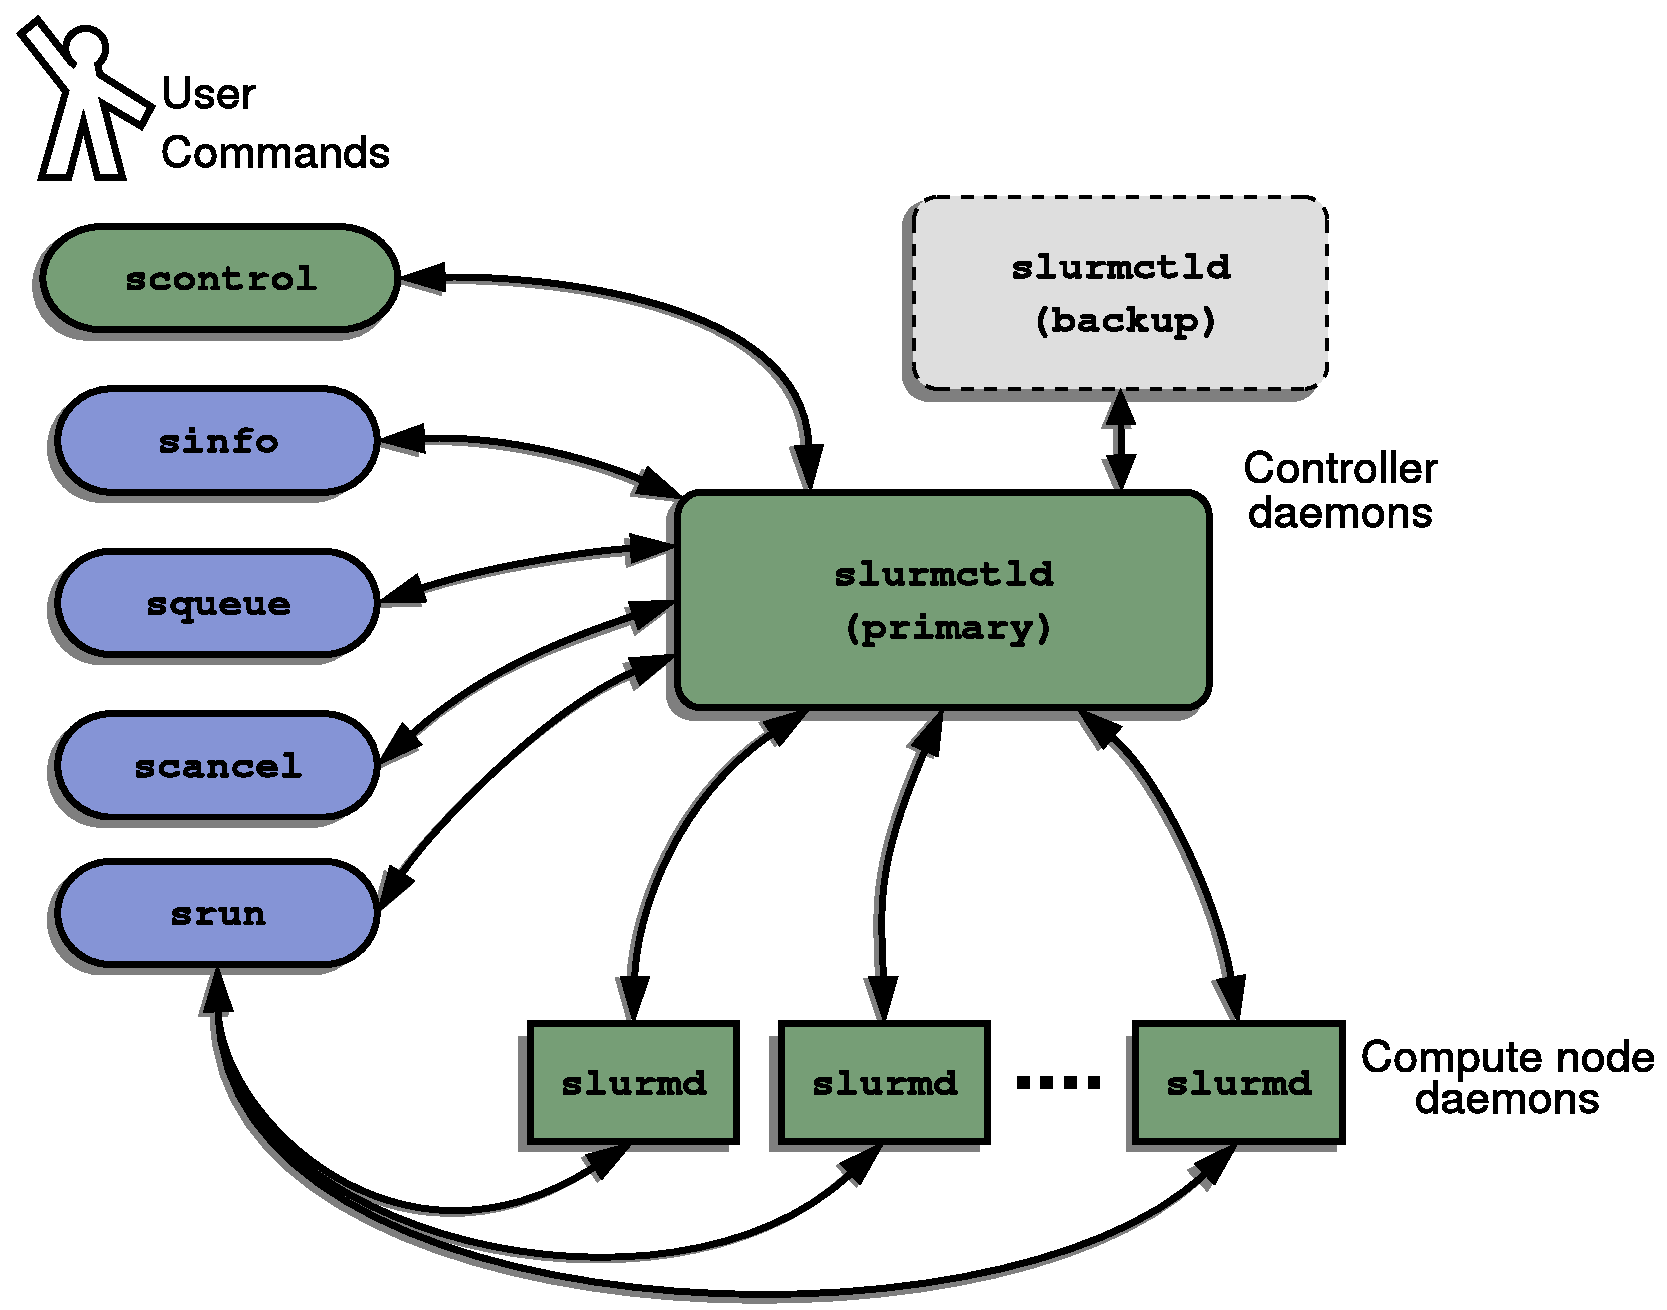
\epsfig{file=../figures/arch.eps,scale=0.35}}
\caption{\small SLURM architecture}
\label{arch}
\end{figure}

As shown in Figure~\ref{arch}, SLURM consists of a \slurmd\ daemon
running on each compute node, a central \slurmctld\ daemon running
on a management node (with optional fail-over twin), and five command
line utilities: \srun\, \scancel, \sinfo\, \squeue\, and \scontrol\, 
which can run anywhere in the cluster.

The central controller daemon, \slurmctld\, maintains the global
state and directs operations.
\slurmctld\ monitors the state of nodes (through {\tt slurmd}),
groups nodes into partitions with various contraints,  
manages a queue of pending work, and
allocates resouces to pending jobs and job steps.
\slurmctld\ does not directly execute any user jobs, but 
provides overall management of jobs and resources.
  
Compute nodes simply run a \slurmd\ daemon (similar to a remote 
shell daemon) to export control to SLURM.
Each \slurmd\ monitors machine status, 
performs remote job execution, manages the job's I/O, and otherwise 
manages the jobs and job steps for its execution host.

Users interact with SLURM through four command line utilities: 
\srun\ for submitting a job for execution and optionally controlling 
it interactively, 
\scancel\ for signalling or terminating a pending or running job,
\squeue\ for monitoring job queues, and 
\sinfo\ for monitoring partition and overall system state.  
System administrators perform privileged operations through an 
additional command line utility, {\tt scontrol}.

The entities managed by these SLURM daemons include {\em nodes}, the
compute resource in SLURM, {\em partitions}, which group nodes into
logical disjoint sets, {\em jobs}, or allocations of resources assigned
to a user for a specified amount of time, and {\em job steps}, which
are sets of (possibly parallel) tasks within a job.  Each job in the
priority-ordered queue is allocated nodes within a single partition.
Once a job is assigned a set of nodes, the user is able to initiate 
parallel work in the form of job steps in any configuration within 
the job's allocation. 
For instance, a single job step may be started that utilizes all nodes
allocated to the job, or several job steps may independently use a
portion of the allocation.

\begin{figure}[tcb]
\centerline{\epsfig{file=../figures/entities.eps,scale=0.5}}
\caption{\small SLURM entities: nodes, partitions, jobs, and job steps}
\label{entities}
\end{figure}

Figure~\ref{entities} further illustrates the interrelation of these
entities as they are managed by SLURM by showing a group of
compute nodes split into two partitions. Partition 1 is running one job,
with one job step utilizing the full allocation of that job.  The job
in Partition 2 has only one job step using half of the original job
allocation.  That job might initiate additional job steps to utilize
the remaining nodes of its allocation.

In order to simplify the use of different infrastructures,
SLURM uses a general purpose plugin mechanism.  A SLURM plugin is a
dynamically linked code object that is loaded explicitly at run time
by the SLURM libraries.  A plugin provides a customized implementation
of a well-defined API connected to tasks such as authentication,
or job scheduling.  A common set of functions is defined
for use by all of the different infrastructures of a particular variety.
For example, the authentication plugin must define functions such as 
{\tt slurm\_auth\_create} to create a credential, {\tt slurm\_auth\_verify}
to verify a credential to approve or deny authentication, etc.  
When a SLURM command or daemon is initiated, it
reads the configuration file to determine which of the available plugins
should be used.  For example {\em AuthType=auth/munge} says to use the
plugin for munge based authentication and {\em PluginDir=/usr/local/lib}
identifies the directory in which to find the plugin.

\section {Blue Gene/L Specific Resource Management Issues}

Since a BGL base partition is the minimum allocation unit for a job, 
it was natural to consider each one as an independent SLURM node. 
This meant SLURM would manage a very reasonable 128 nodes 
rather than tens of thousands of individual c-nodes.
The \slurmd\ daemon was originally designed to execute on each 
SLURM node to monitor the status of that node, launch job steps, etc. 
Unfortunately BGL prohibited the execute of SLURM daemons within 
the base partitions on any of the c-nodes. 
SLURM was compelled to execute \slurmd\ on one or more 
front-end nodes.
In addition,  the typical Unix mechanism used to interact with a 
compute host (e.g. getting memory size or processor count) do not 
function normally with BGL base partitions. 
This issue was addressed by adding a SLURM parameter to 
indicate when it is running with a front-end node, in which case 
there is assumed to be a single \slurmd\ for the entire system. 
We anticipate changing this in the future to support multiple 
\slurmd\ daemons on the front-end nodes.

SLURM was originally designed to address a one-dimensional topology
and this impacted a variety of areas from naming convensions to 
node selection. 
SLURM provides resource management on several Linux clusters 
exceeding 1000 nodes and it is impractical to display or otherwise 
work with hundreds of individual node names. 
SLURM addresses this by using regular expressions to indicate 
ranges of node names. 
For example, "linux[0-1023]" was used to represent 1024 nodes 
with names having a prefix of "linux" and a numeric suffic ranging 
from "0" to "1023" (e.g. "linux0" through "linux1023"). 
The most reasonable way to name the BGL nodes seemed to be 
using a three digit suffix, but rather than indicate a monotonically 
increasing number, each digit would represent the base partition's 
location in the X, Y and Z dimensions (the value of X ranges 
from 0 to 7, Y from 0 to 3, and Z from 0 to 3 on the LLNL system).
For example, "bgl012" would represent the base partition at
the position X=0, Y=1 and Z=2.
Since BGL resources naturally tend to be rectangular prisms in 
shape, we modified the regular expression to indicate the two 
extreme base partition locations. 
The name prefix is always "bgl". 
Within the brackets one lists the base partition with the smallest
X, Y and Z coordinates followed by a "x" followed by the base 
partition with the highest X, Y and Z coordinates.
For example, "bgl[200x311]" represents the following eight base 
partitions: bgl200, bgl201, bgl210, bgl211, bgl300, bgl301, bgl310
and bgl311.
Note that this method does can not accomodate blocks of base 
partitions that wrap over the torus boundaries particularly well, 
although a regular expression of this sort is supported: 
"bgl[000x-011,700x711]".

The node selection functionality is another topology aware 
SLURM component. 
Rather than embedding BGL-specific logic into a multitude of 
locations, all of this logic was put into a single plugin. 
The pre-existing node selection logic was put into a plugin 
supporting typical Linux clusters with node names based 
upon a one-dimensional array. 
The BGL-specific plugin not only selects nodes for pending jobs 
based upon BGL topography, but issues the BGL-specific APIs 
to monitor the system health (draining nodes with any failure 
mode) and perform initialization and termination sequences for the job.

BGL's topology requirement necessitated the addition of several 
\srun\ options: {\em --geometry} to specify the dimension required by 
the job,
 {\em --no-rotate} to indicate of the geometry specification could rotate 
in three-dimensions,
{\em --comm-type} to indicate the communctions type being mesh or torus,
{\em --node-use} to specify if the second process on a c-node should 
be used to execute the user application or be used for communications. 
While \srun\ accepts these new options on all computer systems, 
the node selection plugin logic is used to manage this data in an 
opaque data type. 
Since these new data types are unused on non-BGL systems, the 
functions to manage them perform no work. 
Other computers with other topology requiremens will be able to 
take advantage of this plugin infrastructure with minimal effort.

In order to provide users with a clear view of the BGL topology, a new 
tools was developed.
\smap\ presents the same type of information as the \sinfo\ and \squeue\ 
commands, but graphically displays the location of SLURM nodes 
(BGL base partitions) assigned to partitions or partitions as shown in 
Table ~\ref{smap_out}.

\begin{table}[t]
\begin{center}

\begin{tabular}[c]{c}
\\
\fbox{ 
   \begin{minipage}[c]{1.0\linewidth}
     {\scriptsize \verbatiminput{smap.output} } 
   \end{minipage} 
}
\\
\end{tabular}
\caption{\label{smap_out} Output of \srun\ command}
\end{center}
\end{table}

Rather than modifying SLURM to initiate and manage the parallel 
tasks for BGL jobs, we decided utilize existing software from IBM. 
This eliminated a multitude of software integration issues. 
SLURM will manage resources, select resources for the job, 
set an environment variable BGL\_PARTITION\_ID, and spawn 
a script. 
The job will initiate its parallel tasks through the use of {\em mpirun}.
{\em mpirun} uses BGL-specific APIs to launch and manage the 
tasks. 
We disabled SLURM's job step support for normal users to 
mitigate the possible impact of users inadvertently attempting 
to initiate job steps through SLURM.

\section{Blue Gene/L Network Wiring Issues}

TBD

Static partitioning

\section{Results}

TBD

\section{Future Plans}

Dynamic partitioning

\raggedright
% make the bibliography
\bibliographystyle{splncs}
\bibliography{project}

% make the back cover page
%\makeLLNLBackCover
\end{document}
